         \chapter{Units used in the book}
    \setcounter{figure}{1}
    \setcounter{subfigure}{1}
    \label{m38491}
\section{ Introduction}
            \nopagebreak
%            \label{m38491*cid1} $ \hspace{-5pt}\begin{array}{cccccccccccc}   \end{array} $ \hspace{2 pt}\raisebox{-0.2em}{
\includegraphics[height=1em]{../icons/www.pdf}} {(section shortcode: P10115 )} \par 
\label{m38491*id5632}A laboratory (be it for physics, chemistry or other sciences) can be a very dangerous and daunting place. However, if you follow a few simple guidelines you can safely carry out experiments in the lab without endangering yourself or others around you.
\par 
\section{Laboratory apparatus}
Listed here are some of the common pieces of apparatus that you will be working with in the lab. You should be able to name all the apparatus listed here as well as make a simple sketch of it. 
\begin{itemize}
 \item Beaker 
\item Flasks
\item Test tubes
\item Bunsen burner
\item Measuring cylinder
\item Pipette
\item Propette
\item Watch glass
\item retort stand
\item thermometer
\item mass meter
\item tripod
\item wire gauze
\item funnel
\item syringe
\item delivery tubes 
\end{itemize}

\section{ General safety rules}
            \nopagebreak
%            \label{m38491*cid2} $ \hspace{-5pt}\begin{array}{cccccccccccc}   \end{array} $ \hspace{2 pt}\raisebox{-0.2em}{
\includegraphics[height=1em]{../icons/www.pdf}} {(section shortcode: P10116 )} \par 
\label{m38491*id7342}The following are some of the general guidelines and rules that you should always observe when working in a laboratory.
\label{m38491*id634222}\begin{enumerate}[noitemsep, label=\textbf{\arabic*}. ] 
            \label{m38491*id632}\item Do not eat or drink in the lab. Do not use lab glassware to eat or drink from.
\label{m38491*id6124}\item Always behave responsibly in the lab. Do not run around or play practical jokes.
\label{m38491*id6342}\item In case of accidents or chemical spills call your teacher at once.
\label{m38491*id7324}\item Always check with your teacher how to dispose of waste. Chemicals should not be disposed of down the sink.
\label{m38491*id632324}\item Only perform the experiments that your teacher instructs you to. Never mix chemicals for fun.
\label{m38491*id6242313}\item Never perform experiments alone. 
\label{m38491*id5512}\item Always check the safety data of any chemicals you are going to use. 
\label{m38491*id523465}\item Follow the given instructions exactly. Do not mix up steps or try things in a different order.
\label{m38491*id73221}\item Be alert and careful when handling chemicals, hot glassware, etc.  
\label{m38491*id5621}\item Ensure all bunsen burners are turned off at the end of the practical and all chemical containers are sealed.
\item Never add water to acid. Always add the acid to water.
\item Never heat thick glassware as it will break. (i.e. do not heat measuring cylinders).
\item When you are smelling chemicals, place the container on a lab bench and use your hand to gently waft (fan) the vapours towards you.
\item Do not take chemicals from the lab.
\item Always work in a well ventilated room. Whenver you perform experiments, you should open the windows.
\item Do not leave bunsen burners and flames unattended. 
\item Never smell, taste or touch chemicals unless instructed to do so.
\item Never point test tubes at people or yourself. When heating chemicals, always point the mouth of the test tube away from you and your classmates.
\end{enumerate}
\par 
\section{ Hazard signs}
            \nopagebreak
%            \label{m38491*eip-411} $ \hspace{-5pt}\begin{array}{cccccccccccc}   \end{array} $ \hspace{2 pt}\raisebox{-0.2em}{
\includegraphics[height=1em]{../icons/www.pdf}} {(section shortcode: P10117 )} \par \label{m38491*eip-990}The table below lists some of the common hazards signs that you may encounter. You should know what all of these mean.
\begin{table}[H]
 \begin{center}
  \begin{tabular}{|l|c|p{3cm}|l|c|p{3cm}|}\hline
   \textbf{Sign} & \textbf{Symbol} & \textbf{Meaning} & \textbf{Sign} & \textbf{Symbol} & \textbf{Meaning} \\ \hline
\parbox[c]{4em}{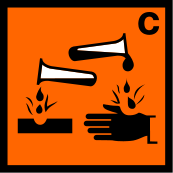
\includegraphics[width=.1\textwidth]{photos/corrosive.png}} & C & Corrosive. Chemicals with this label can burn your skin and eyes and burn holes in your clothes. An example is hydrochloric acid. & \parbox[c]{4em}{
\includegraphics[width=.1\textwidth]{photos/environment.png}} & N & Environmentally harmful. Chemicals with this label are damaging to the environment. An example is CFC's. \\ \hline 
\parbox[c]{4em}{
\includegraphics[width=.1\textwidth]{photos/explosive.png}} & E & Explosive. Chemicals with this label explode easily. An example is lead azide. & \parbox[c]{4em}{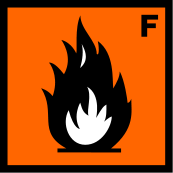
\includegraphics[width=.1\textwidth]{photos/flammable.png}} & F & Flammable. Chemicals with this label can catch fire easily. Example: methanol \\ \hline 
\parbox[c]{4em}{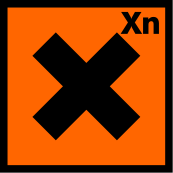
\includegraphics[width=.1\textwidth]{photos/harmful.png}} & Xn & Harmful. Chemicals labeled with this are generally considered to be damamging to humans. & \parbox[c]{4em}{
\includegraphics[width=.1\textwidth]{photos/irritant.png}} & Xi & Irritant. Chemicals with this label cause irritation to your eyes and skin. An example is hydrogen peroxide. \\ \hline 
\parbox[c]{4em}{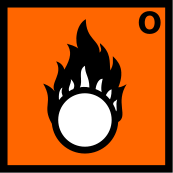
\includegraphics[width=.1\textwidth]{photos/oxidise.png}} & O & Oxidising. Chemicals with this label contain oxygen that may cause other materials to combust. An example is potassium dichromate. & \parbox[c]{4em}{
\includegraphics[width=.1\textwidth]{photos/toxic.png}} & T & Toxic. Chemicals with this label are highly toxic. An example is mercury. \\ \hline 
  \end{tabular}
 \end{center}
\end{table}
      \par \section{ Notes and information}
            \nopagebreak
%            \label{m38491*eip-475} $ \hspace{-5pt}\begin{array}{cccccccccccc}   \end{array} $ \hspace{2 pt}\raisebox{-0.2em}{
\includegraphics[height=1em]{../icons/www.pdf}} {(section shortcode: P10118 )} \par \label{m38491*eip-86}
You can find safety data sheets at Merck\footnote{http://www.merck-chemicals.co.za/safety-data-sheets/c\_O\_Sb.s1LQz0AAAEWVOYfVhTo}. You should always look at these data sheets anytime you work with a new chemical. These data sheets contain information about how to work with chemicals and what dangers the chemicals pose to you and the environment.
\par 
\label{m38491*id7322}You should always try dispose of chemicals correctly and safely. Many chemicals cannot simply be washed down the sink. 
\par 
\label{m38491**end}
      \newpage 
      \def\leftmark{GLOSSARY}
      \def\rightmark{GLOSSARY}
      \begin{indexheading}
